% replace all text with your own text.
% in this template few examples are mention
\chapter{Methodology}
\label{ch:method} % Label for method chapter

\subsubsection{{Data Collection and Preprocessing}}

The dataset utilized in this research, referred to as the ISOT Fake News \cite{fake-news}, encompasses articles categorized as either authentic or fabricated news. The data gathering process involved several key steps: authentic news articles were procured through web crawling from Reuters.com, a renowned news platform acclaimed for its credibility, while fabricated news articles were sourced from multiple untrustworthy outlets identified by Politifact, a prominent fact-checking entity, and Wikipedia. To maintain uniformity, articles were predominantly collected within the timeframe of 2016 to 2017. The dataset comprises two CSV files: "True.csv" containing over 12,600 articles sourced from Reuters.com and "Fake.csv" containing a similar number of articles from diverse fake news sources. Each article within the dataset includes essential information such as the title, text, type (real or fake), and publication date. 

 \begin{figure}

     \centering
     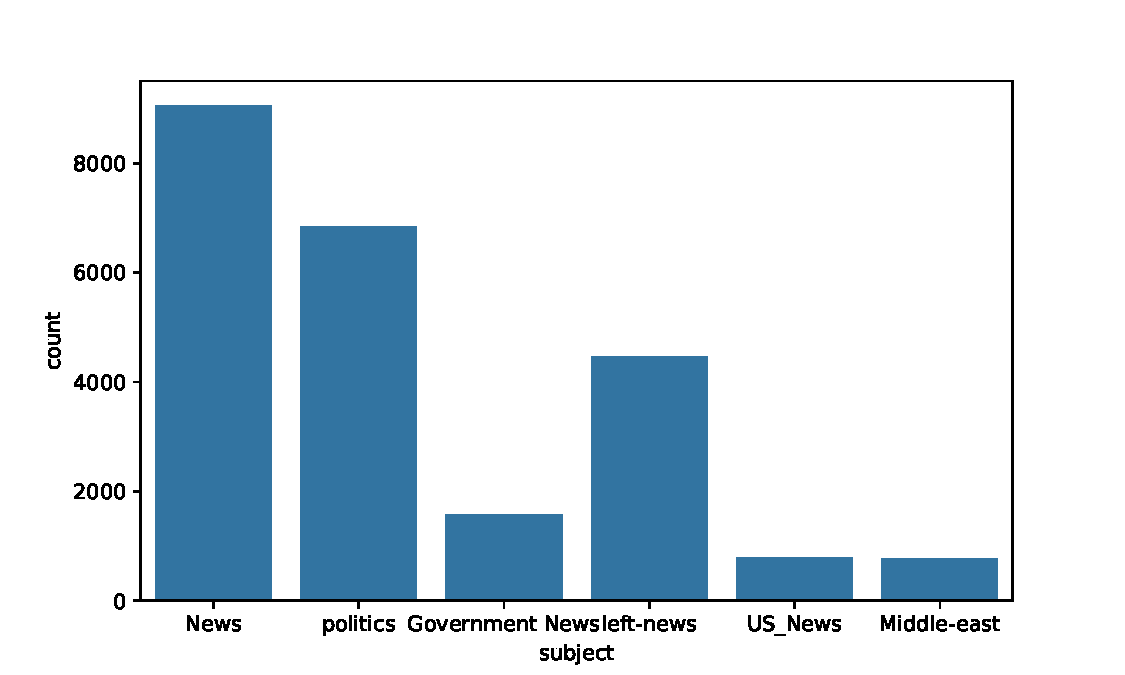
\includegraphics[width=1\linewidth]{figures/FakeNewCategories.pdf}
     \caption{Fake News Categories}
     \label{fig:enter-label}
 \end{figure}

\begin{figure}
    \centering
    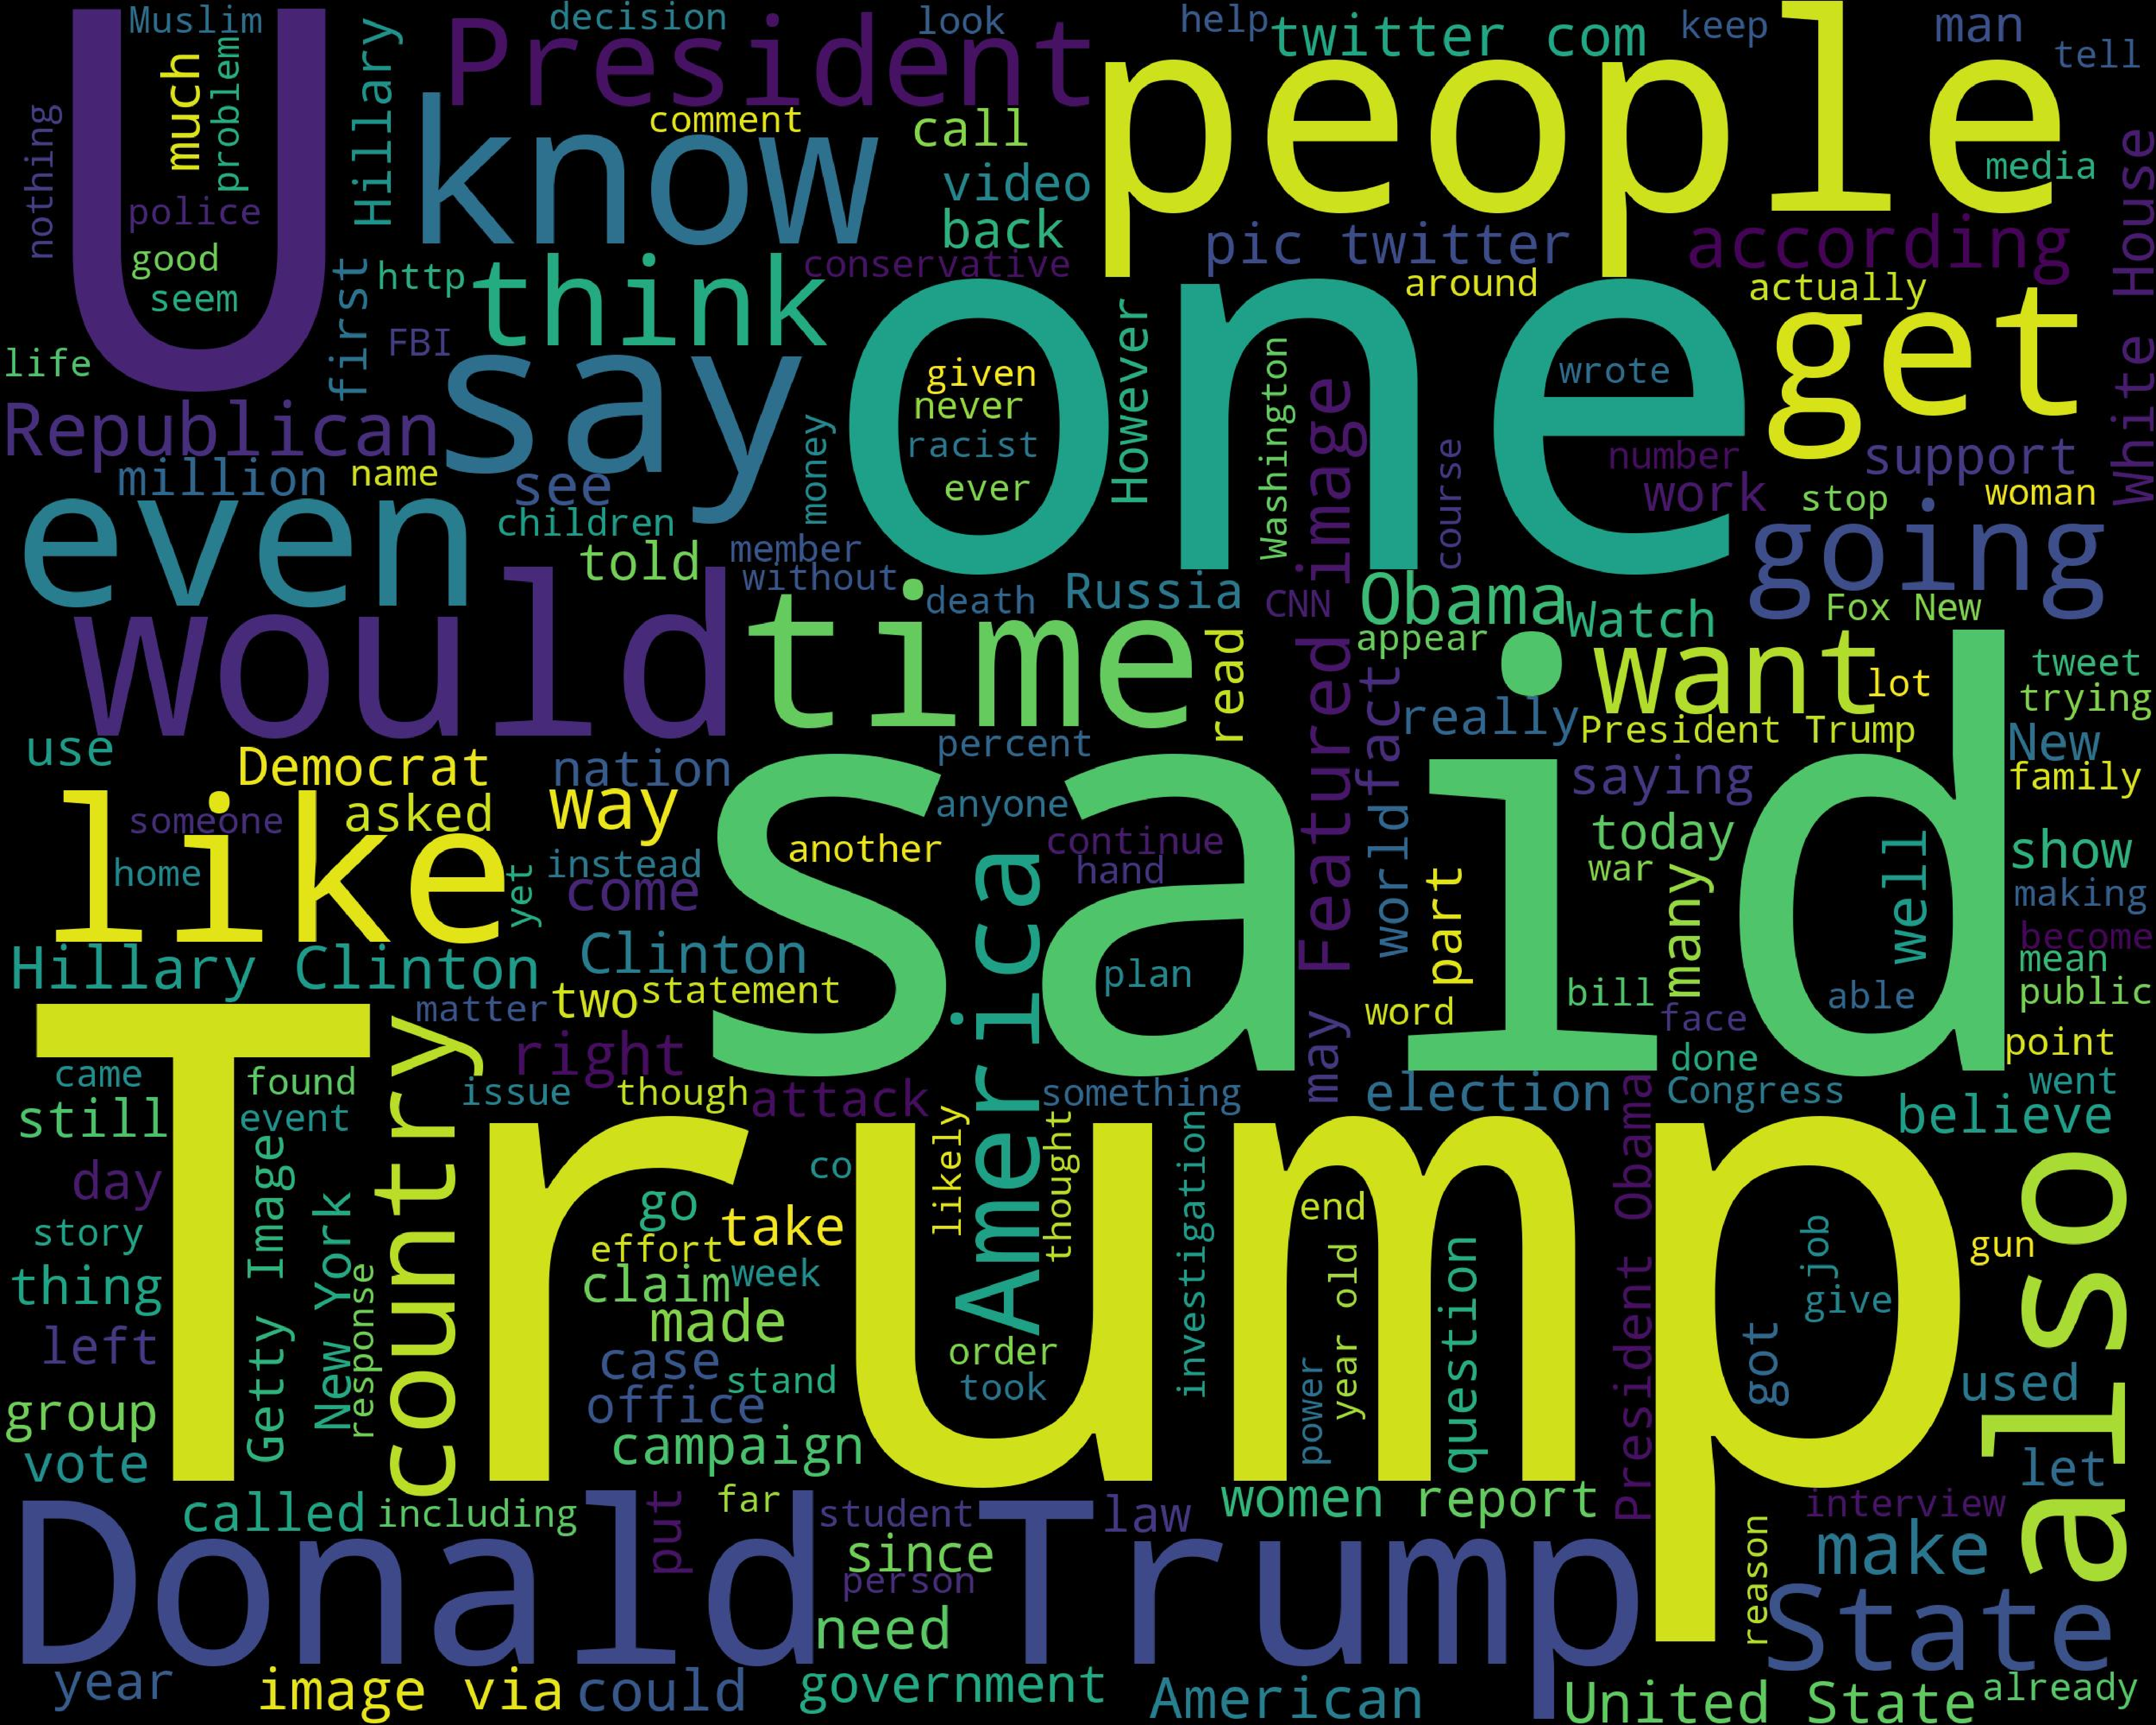
\includegraphics[width=0.75\linewidth]{figures/fakenews_wordcloud.pdf}
    \caption{Fake News - word Cloud}
    \label{fig:enter-label}
\end{figure}
\subsubsection{{Exploratory Data Analysis (EDA)}}

We performed Exploratory Data Analysis (EDA) on the preprocessed dataset to gain insights into the distribution of real and fake news articles, as well as the distribution of news articles across different subjects. The following figures were generated to visualize the dataset:

 